\documentclass[10.5pt,compsoc,UTF8]{CjC}
% CjC.cls defines its own Chinese size macro, while current CTeX also defines
% \zihao. Preserve the CjC definitions, temporarily undefine the collision
% while loading the installed CTeX package, then restore the CjC size map.
\RequirePackage{expl3}
\let\CjCzihao\zihao
\let\CjCnormalSize\normalsize
\let\normalsize\relax
\ExplSyntaxOn
\cs_undefine:N \zihao
\ExplSyntaxOff
\RequirePackage{ctex}
\let\zihao\CjCzihao
\let\normalsize\CjCnormalSize

\RequirePackage{amsmath,amssymb}
\RequirePackage{etoolbox}
\RequirePackage{booktabs,tabularx,array}
\RequirePackage{float}
\RequirePackage{graphicx}
\RequirePackage{gbt7714}
\citestyle{super}
\RequirePackage{stfloats}
\RequirePackage{cuted}
\RequirePackage{captionhack}
\makeatletter
\renewcommand{\fnum@figure}{{\zihao{5-}\textbf{图\thefigure}}}
\renewcommand{\fnum@table}{{\zihao{5-}\textbf{表\thetable}}}
\makeatother
\RequirePackage{hyperref}
\hypersetup{hidelinks}
\graphicspath{{figures/}}
\setmainfont{TeX Gyre Termes}
\renewcommand{\figurename}{图}
\renewcommand{\tablename}{表}
\AtBeginEnvironment{thebibliography}{\footnotesize\interlinepenalty=10000}
% The source SVGs contain a small unused bottom canvas margin; the figure
% environments trim that margin. Keep the remaining caption gap compact.
\setlength{\abovecaptionskip}{4pt}
\setlength{\belowcaptionskip}{0pt}
\setlength{\parindent}{2em}
\setlength{\columnsep}{8mm}
\setlength{\emergencystretch}{1em}
\renewcommand{\theequation}{\arabic{equation}}
\newlength{\CjCAbstractSideIndent}
\setlength{\CjCAbstractSideIndent}{\parindent}
\newlength{\CjCAbstractAfterSkip}
\setlength{\CjCAbstractAfterSkip}{6mm}

\providecommand{\tightlist}{%
  \setlength{\itemsep}{0pt}\setlength{\parskip}{0pt}}




% A4 single-column course-paper layout.
\RequirePackage{geometry}
\geometry{a4paper,left=24mm,right=24mm,top=45mm,bottom=18mm,headheight=17pt,headsep=8mm,footskip=11mm}
\RequirePackage[section]{placeins}
\renewcommand{\baselinestretch}{1.25}
\renewcommand{\normalsize}{\fontsize{11pt}{15.6pt}\selectfont}
\renewcommand{\small}{\fontsize{9.5pt}{13.1pt}\selectfont}
\renewcommand{\footnotesize}{\fontsize{8.5pt}{11.5pt}\selectfont}
\AtBeginDocument{\normalsize}
\setlength{\parindent}{2em}
\setlength{\parskip}{0pt}
\setlength{\abovedisplayskip}{7pt plus 2pt minus 2pt}
\setlength{\belowdisplayskip}{7pt plus 2pt minus 2pt}
\setlength{\textfloatsep}{11pt plus 3pt minus 2pt}
\setlength{\intextsep}{10pt plus 3pt minus 2pt}
\setcounter{topnumber}{3}
\renewcommand{\topfraction}{0.9}
\renewcommand{\textfraction}{0.08}
\renewcommand{\floatpagefraction}{0.7}
\raggedbottom


\newcommand{\PaperTitleCN}{分布式 MoE 训练中的动态专家与样本放置机制研究}
\newcommand{\PaperTitleEN}{Dynamic Expert and Sample Placement in Distributed MoE Training}
\newcommand{\AuthorName}{黄泓霖}
\newcommand{\AuthorNameEN}{[To be filled]}
\newcommand{\StudentNumber}{2600671011}
\newcommand{\DepartmentName}{人工智能}
\newcommand{\MajorName}{智能科学与技术}
\newcommand{\CourseName}{下一代互联网技术}
\newcommand{\InstructorName}{李雪亮}
\newcommand{\SubmissionDate}{12月10日}
\newcommand{\HeaderText}{下一代互联网技术课程论文}


\headevenname{\HeaderText}
\headoddname{\PaperTitleCN}
\pagestyle{CjCheadings}

\begin{document}
\setcounter{page}{1}

\begin{center}
{\zihao{2}\heiti \PaperTitleCN\par}
\vspace{3mm}
{\zihao{4}\fangsong 作者：\AuthorName\quad 学号：\StudentNumber\par}
\vspace{1mm}
{\zihao{5-} 学院与专业：\DepartmentName / \MajorName\quad 课程：\CourseName\par}
{\zihao{5-} 任课教师：\InstructorName\quad 提交日期：\SubmissionDate\par}
\end{center}
\vspace{1mm}
\noindent\hspace*{\CjCAbstractSideIndent}\begin{minipage}{\dimexpr\textwidth-2\CjCAbstractSideIndent\relax}
{\zihao{5-}\setlength{\baselineskip}{13.5pt}\selectfont
\noindent{\heiti 摘要\quad}
分布式 MoE 训练将专家分散到多张 GPU，扩大了模型容量，但也使 token 分发与回收产生跨设备 All-to-All 通信。现有研究分别通过 expert fetch、动态专家复制和 sample placement 缓解通信路径或专家热点，但三者作用的资源并不相同。本文以关键路径上的暴露等待为分析视角，比较这些机制的收益来源、调整成本和适用负载，指出样本放置主要改善网络局部性，专家复制主要缓解持续性计算或容量热点，专家拉取则通过改变通信对象减少特定条件下的数据搬运。基于这一判断，本文提出一种面向主导瓶颈识别的自适应放置思路，并给出区分控制变量测试与端到端训练效果的验证方案。\par
\vspace{1mm}
\noindent{\heiti 关键词\quad}混合专家模型；分布式训练；专家并行；All-to-All；动态专家放置；样本放置；Scale-out\par}
\end{minipage}

\vspace{\CjCAbstractAfterSkip}

\section{引言与技术背景}
\label{sec:introduction}

\subsection{分布式 MoE 训练的通信瓶颈}

Mixture-of-Experts（MoE）通过路由器为每个 token 选择 Top-1 或 Top-2 个 expert，使模型在不按比例增加单 token 计算量的情况下扩大参数规模。在专家并行中，不同 GPU 保存不同专家；如果 token 所在 GPU 与目标专家不一致，系统就要发送 hidden state，执行专家计算，再把结果返回原来的计算流，反向阶段还需沿专家路由回传输入梯度；如存在专家副本，其参数梯度的汇总或同步取决于具体并行方案。这一前向分发、专家计算和结果回收过程通常表现为 All-to-All，而不是所有 GPU 共享同一结果的 All-Reduce。NetMoE 指出，一个 MoE 层在一次前向与反向迭代中可能涉及四次 All-to-All\cite{ref3}。

在 Scale-out 集群中，机内 NVLink、NVSwitch 或 PCIe 与跨节点链路的带宽和延迟不同，动态路由又使通信矩阵随输入变化。token 访问远端专家时可能产生跨节点传输等待，热门专家可能引起计算排队；专家容量受限时还可能造成 Token Dropping。Janus 在 16 与 32 张 A100 的多组 MoE 训练实验中报告，All-to-All 通信时间占单次迭代时间的 38.5\%--68.4\%\cite{ref1}。因此训练延迟并非显卡矩阵乘法时间的简单总和，通信路径和专家负载都可能成为瓶颈。

\subsection{静态专家放置的局限性}

固定专家、移动 token 会同时暴露两类压力：位置不匹配造成跨节点搬运，热门专家可能排队，容量受限还会造成 token dropping。扩大容量可以减少 token 丢弃，却可能增加填充和无效计算；提高负载均衡辅助损失项的权重虽能改善负载，也可能改变专家专门化。FlexMoE 的 Swin-MoE 例子显示，负载均衡辅助损失项的系数（balance loss coefficient）从 0 调至 0.05 时，GPU 利用率由 18.77\% 提升到 63.30\%，Top-5 准确率由 94.588\% 变为 93.981\%\cite{ref2}。

增加网络带宽只能直接缓解传输，路由平衡也不能保证 token 已经靠近目标专家。静态布局没有根据路由局部性和专家热度变化重新安排数据与计算位置，而不仅是网络带宽不足，这构成了研究动态放置机制的动机。

\subsection{动态放置机制与性能影响因素}

Janus 按需拉取专家权重改变通信对象；FlexMoE、SYMI 调整专家实例数量或位置缓解负载；NetMoE 利用同一样本中 token 的路由偏好，调整样本节点与设备归属，利用机内外通信差异。这些策略受状态同步、权重搬运、映射维护、求解、显存和计算通信重叠成本约束。

核心问题是：在不同的局部性、专家热点和调整窗口下，专家拉取、专家复制与样本放置分别解决什么关键路径瓶颈，哪一种动作更可能获得端到端净收益？第 2 章比较代表性工作，第 3 章提炼未解决的矛盾，第 4 章提出个人研究思路及验证方法。图~\ref{fig:overview} 概览分布式 MoE 训练中的系统组成、静态放置挑战和动态放置主线。

\begin{figure}[!htbp]
\centering
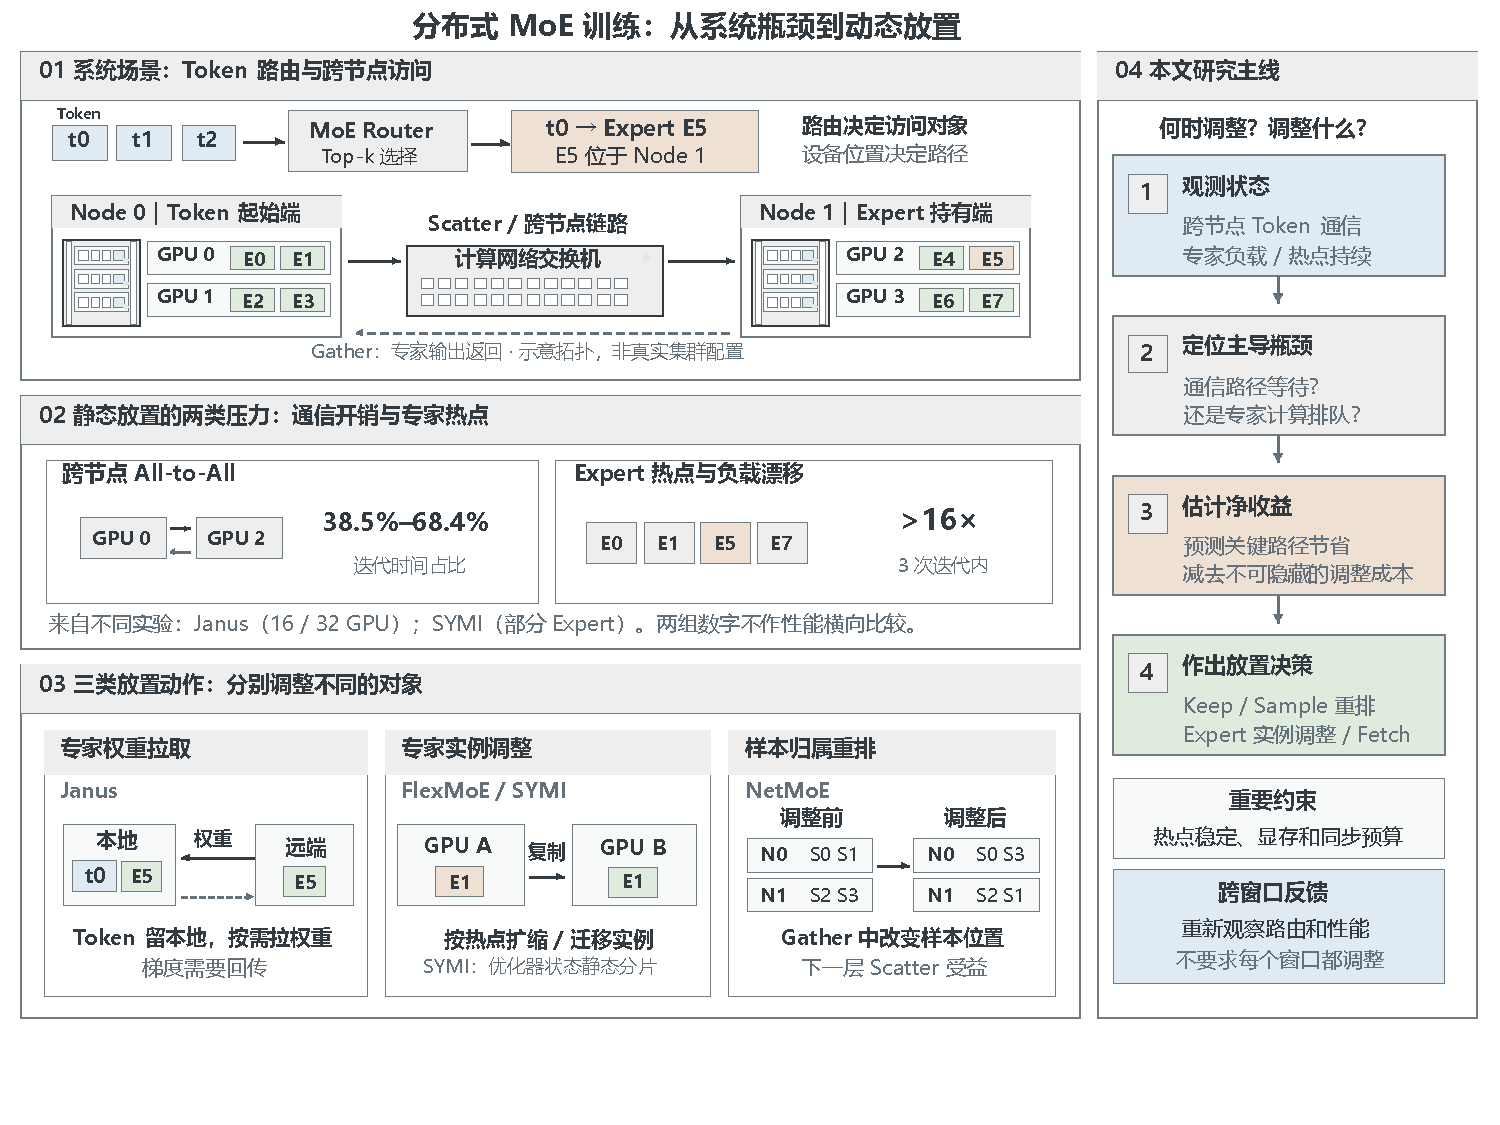
\includegraphics[width=\linewidth,trim=0 46pt 0 0,clip]{figures/figure1.pdf}
\caption{分布式 MoE 训练系统与动态放置研究主线。面板 01 为拓扑示意，面板 04 为研究设想；面板 02 的数字不作同配置比较。根据 Janus\cite{ref1}、NetMoE\cite{ref3}、SYMI\cite{ref4} 等文献整理绘制。}
\label{fig:overview}
\end{figure}


\section{动态放置机制的研究进展与比较}
\label{sec:research}

\subsection{基于专家拉取的数据中心化训练}

Janus\cite{ref1}首先重新选择了通信对象。固定专家方式移动大量 token 或 activation，Janus 则让数据保留在原 worker，根据当前路由按需拉取对应专家权重，并用缓存、机内共享、预取、拓扑优先级和异步任务重叠通信与计算。其成立的关键条件是，需要传输的 token 数据量大于可复用的专家权重，并且权重拉取不会因拷贝和调度产生新的暴露等待。

在 32 张 A100 上，Janus 报告最多 16 倍流量减少和 2.06 倍迭代加速\cite{ref1}。这些结果支持``改变通信对象能够改变网络代价''的判断，但 Janus 的机制是按需取得计算所需的权重，而非把热门 expert 永久迁移或复制到更多 GPU：反向阶段仍要把梯度送回原始 worker。因此，专家尺寸、batch 或 sequence 规模、权重复用和缓存命中情况决定了拉取是否有利；当权重不再小于需要交换的 token 时，原有以专家为中心的通信方式可能重新具有竞争力。

\subsection{面向负载均衡的动态专家放置}

FasterMoE、FlexMoE 和 SYMI 面向的是热门 expert 造成的计算、容量和排队压力。FasterMoE 用性能模型和 DDL-Roofline 判断何时对热门专家做 shadowing，并把 All-to-All 与专家计算拆成可重叠任务\cite{ref5}。FlexMoE 将扩展、收缩和迁移纳入放置决策，通过增加热门专家副本分摊 token；其 64 张 A100 实验相对 DeepSpeed 平均 1.70 倍、最高 2.10 倍，相对 FasterMoE 平均 1.30 倍、最高 1.45 倍\cite{ref2}。两类方法的收益来源都是增加热门专家的可用计算槽位，而不是直接让所有 token 留在本地。

副本扩张随之引入状态问题：权重需要分发，副本梯度需要同步，迁移还可能涉及优化器状态；若热点持续时间过短，重配置成本可能无法被后续收益摊销。

专家容量还关联 token dropping 和训练收敛。SYMI 的 16-GPU GPT-Small 设置中，容量系数为 ×1、×2、×4 时，token survival 分别为 44.90\%、65.56\%、74.91\%，达到目标 loss 分别需要 618、527、478 次迭代，前向延迟为 455.41、506.77、571.42 ms\cite{ref4}。这表明专家复制的评价不能只看单步时间，还要同时观察 token 接纳率和训练进展。

SYMI 把优化器状态静态分片，同时根据 popularity 调整 GPU 上的专家权重或实例放置，降低状态随专家移动的约束。该结果体现状态解耦与动态放置的结合，不意味着副本不再需要权重、梯度或集合通信；其设计复用了正常优化器更新中本来就要发送的更新权重。论文在 16 张 A100 GPU 的评测中报告，GPT-Small 达到 loss 4.0 时，DeepSpeed 为 147.84 分钟，SYMI 为 102.68 分钟；相对 DeepSpeed 和 FlexMoE 的 time-to-convergence 分别快 30.5\% 和 25.9\%，并报告相对系统少丢 43\%--69\% 的 token\cite{ref4}。这些结果不能归因于单一因素。

\subsection{基于路由局部性的动态样本放置}

NetMoE\cite{ref3}从样本一侧处理跨节点路径。它利用同一样本的 token 可能具有路由局部性，先决定样本的节点，再决定节点内设备，使部分 token 在目标节点内完成后续交换。NetMoE 不先执行独立的跨节点样本迁移，而是把新的设备分配融合到当前层 All-to-All Gather，使专家输出直接落到新的样本位置；由于该位置会成为下一层输入，优化目标同时包含当前层 Gather 与下一层 Scatter。

为保证重排不破坏 Transformer 的残差语义，NetMoE 使用 expert residual inlining，将残差加法安排在 Scatter 之后、Gather 之前。为满足在线训练的时间要求，它将放置求解转化为加权二分图匹配，用 Kuhn-Munkres 在 CPU 后台运行，并与 scatter 和专家计算重叠。因而主要代价是既有 Gather/下一层 Scatter 的目的地重定向、索引与残差映射维护及匹配求解，而不是额外的大规模搬运。

在 4 节点、32 张 A800-SXM4 40 GB 的实验中，NetMoE 在 50 次迭代平均设置下最高相对 FastMoE、FasterMoE 和 SmartMoE 加速 1.67、1.37 和 1.33 倍；在 Table 4 的 MoE-GPT-S、16 GPU、I/J=2 求解器对比中，KM 为 0.08 ms、PuLP 为 42.8 ms\cite{ref3}，不等同于上一句 32 GPU 实验的通用开销。样本位置可用于网络优化，但重排不消除 All-to-All：它仍需维护样本、序列、残差和微批对应关系，只在局部性和机内外带宽差异存在时减少跨节点部分。

\subsection{不同动态放置机制的综合比较}

三类放置对象的差别在于移动对象和释放资源：专家拉取改变数据与权重的交换对象，专家复制增加热门专家的计算位置，样本重排改善 token 与 expert 的拓扑映射；通信调度是可叠加的执行层，调整已有通信顺序。图~\ref{fig:mechanisms} 展示四项工作的决策链路与调整成本。

\begin{figure}[!htbp]
\centering
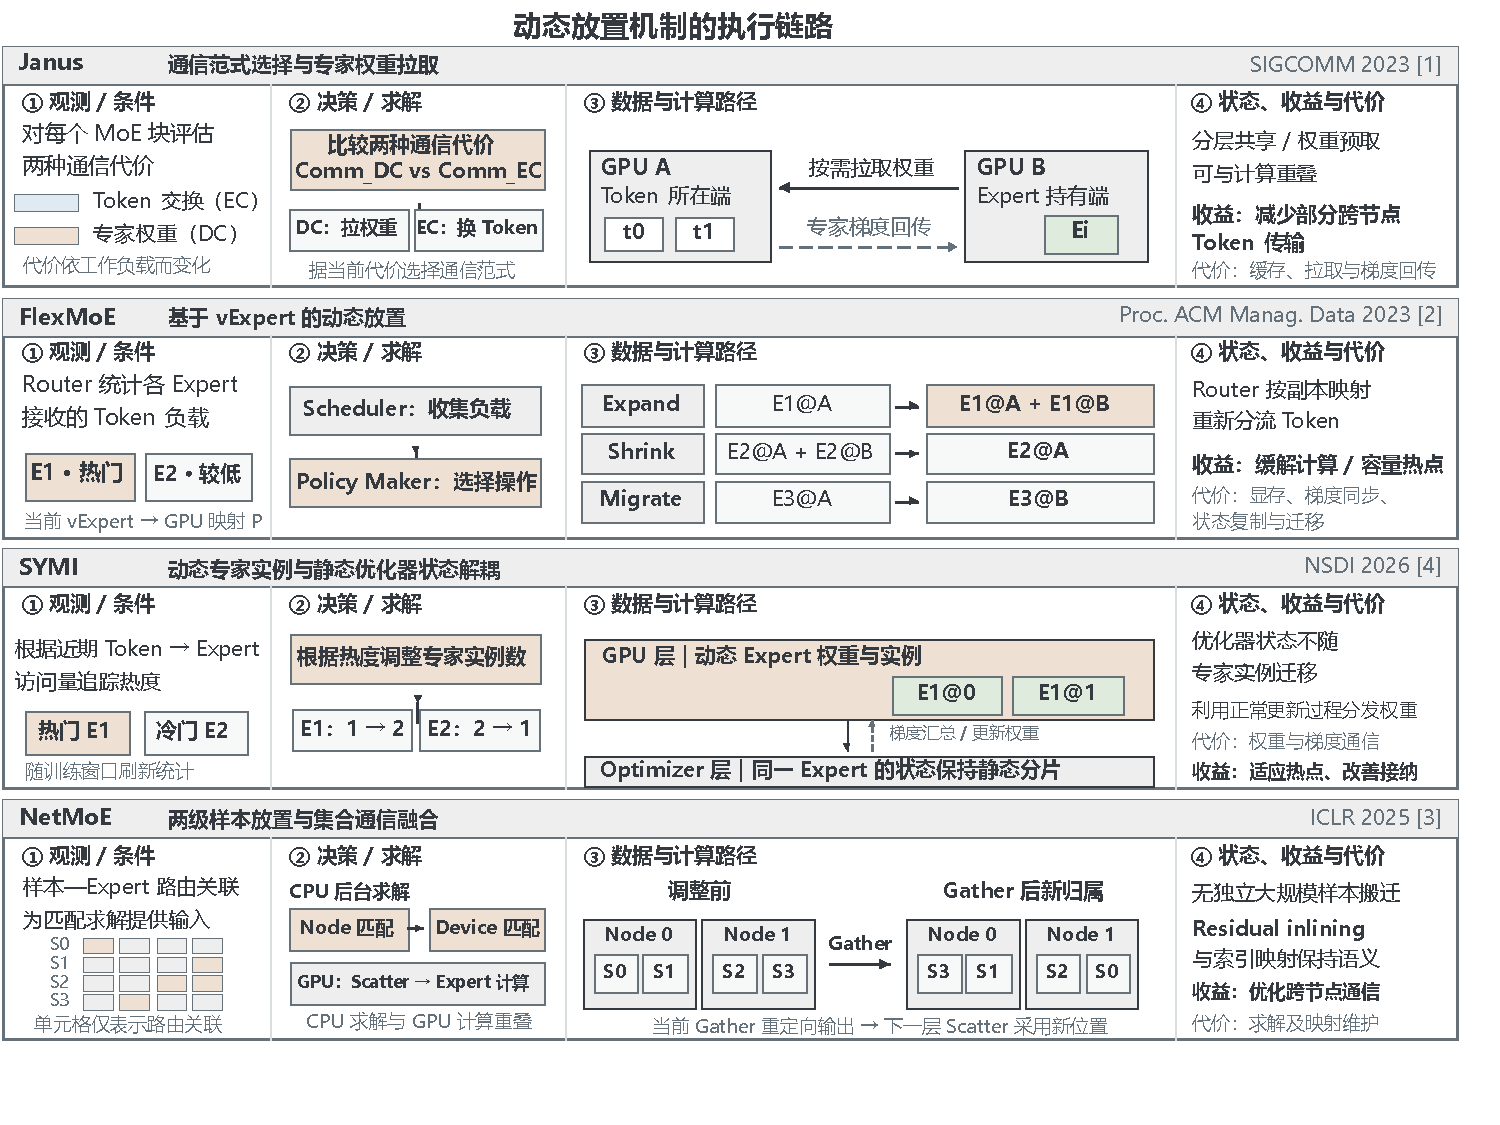
\includegraphics[width=\linewidth,trim=0 36pt 0 0,clip]{figures/figure2.pdf}
\caption{Janus、FlexMoE、SYMI 与 NetMoE 的主要执行链路。Janus 中 EC 表示 expert-centric，DC 表示 data-centric；四条泳道按代表工作组织，不作性能排名。根据文献 \cite{ref1,ref2,ref3,ref4} 整理绘制。}
\label{fig:mechanisms}
\end{figure}

\begin{table}[!t]
\centering
\caption{动态放置机制的条件化比较}
\label{tab:mechanism-comparison}
\footnotesize
\setlength{\tabcolsep}{2pt}
\renewcommand{\arraystretch}{1.12}
\begin{tabularx}{\linewidth}{>{\raggedright\arraybackslash}p{0.12\linewidth} >{\raggedright\arraybackslash}p{0.11\linewidth} >{\raggedright\arraybackslash}p{0.14\linewidth} >{\raggedright\arraybackslash}p{0.12\linewidth} >{\raggedright\arraybackslash}p{0.16\linewidth} >{\raggedright\arraybackslash}p{0.18\linewidth} >{\raggedright\arraybackslash}X}
\toprule
研究类别 & 代表工作 & 改变对象 & 主要瓶颈 & 关键收益来源 & 新增成本 & 典型适用条件 \\
\midrule
数据中心化专家拉取 & Janus\cite{ref1} & 专家权重与缓存位置 & token 跨节点搬运 & 用权重拉取替代部分 token 交换 & 权重搬运、缓存、拷贝、反向梯度回传 & 权重相对 token 数据较小且可复用 \\
动态专家复制/迁移 & FasterMoE\cite{ref5}、FlexMoE\cite{ref2}、SYMI\cite{ref4} & 热门专家副本和状态布局 & 专家计算或容量热点 & 增加热门专家的计算槽位 & 显存、权重更新、梯度同步、状态管理 & 热点持续、同步预算和显存充足 \\
动态样本放置 & NetMoE\cite{ref3} & 样本的节点或设备归属 & 跨节点网络路径 & 提高 token 与 expert 的局部性 & Gather 重定向、下一层 Scatter 联动、求解和映射维护 & 局部性明显、机内外带宽差异大 \\
通信调度与并行优化 & SmartMoE\cite{ref6}、Tutel\cite{ref7}、Lina\cite{ref8}、Parm\cite{ref9} & schedule、pipeline、micro-op & 已存在的通信暴露等待 & 调整并行策略、通信调度与竞争/重叠 & 切分、候选搜索和控制开销 & 放置不宜频繁改变或需作为共同执行层 \\
\bottomrule
\end{tabularx}
\end{table}

上述比较表明，两类局部性与专家负载偏斜并不等同。若路由局部性高且专家负载均衡，主要等待来自 token 的跨节点路径，样本重排更直接；复制专家会增加同步，却未必减少主要等待。若路由局部性低但某一专家在多个窗口持续过热，样本重排难以把随机访问变成本地访问，专家复制更可能缓解计算排队，但不能自动消除 token 传输。因此两类局部性与计算热点应分开诊断。

三类动作的净收益取决于调整能否隐藏：样本重排承担 Gather/Scatter 重定向与映射成本，专家复制需要权重、梯度和显存预算，expert fetch 需要缓存、权重复用与反向回传。只有节省的关键路径时间超过无法隐藏的求解、搬运、同步和切换成本，且局部性或热点足够持续，动态动作才值得执行。固定 routing、token 接纳规则和通信设置不变时，应比较 step-time 净收益；若改变容量与 token dropping，还要比较相同目标质量下的 time-to-convergence。SmartMoE、Tutel、Lina 和 Parm 表明调度可作共同执行层；路由快速变化时，保持布局并优化通信顺序可能更合适。


\section{动态放置机制面临的关键挑战}
\label{sec:challenges}

\subsection{动态路由与专家负载变化的适应性}

路由局部性指同一样本 token 的 expert 选择关联性，网络局部性指样本所在节点或设备与目标 expert 的拓扑邻近程度；两者、expert popularity 和跨节点通信占比均随窗口变化。上一窗口的热点不一定延续，路由局部性也可能与全局专家负载趋势不同；调整过慢会滞后，逐步调整又可能暴露求解和状态更新成本。现有方法分别利用局部性、popularity 或历史工作负载预测，但缺少在同一比较条件下判断两类信号持续性的统一标准。

观测粒度也不同：路由局部性按样本或节点统计，网络局部性按样本设备与目标专家的拓扑关系统计，专家 popularity 按专家和窗口统计，窗口长度并不天然相同。

\subsection{动态调整收益与重配置成本的权衡}

判断是否值得调整，需要估计窗口内能减少多少关键路径等待，以及哪些成本无法被计算隐藏。样本放置的求解和索引、专家副本的权重与梯度同步、SYMI 的优化器状态位置，以及 Janus 的拉取和缓存，都可能改变端到端 step time。现有论文指标各异，缺口在于把暴露等待和调整成本放入同一观察窗口。

若策略还改变 expert capacity 或 token dropping，单步时间不能代表训练总成本：更低延迟可能伴随更多 token 丢弃，最终需要更多迭代达到同一质量。因此还应观察 per-step 暴露时间和 time-to-target-quality。

\subsection{通信局部性与专家负载的协同优化}

针对单一瓶颈的优化可能把等待转移到另一处：减少跨节点字节却未减轻热门专家计算，或复制后计算更均衡却新增副本同步。因此需要研究：系统能否识别主导的是网络路径、专家计算还是调整控制，并在保持现状、样本重排和专家复制之间进行有成本意识的选择？这连接了第 2 章的机制差异与下一章的个人方案。


\section{未来研究方向与个人思考}
\label{sec:future}

\subsection{面向主导性能瓶颈的自适应放置框架}

本文设想一个简洁的自适应放置框架。每个决策窗口记录跨节点 All-to-All 暴露等待、各 expert 负载、sample routing locality、热点持续时间和可用显存，先判断主要约束是网络路径还是持续性专家计算，再评估 sample placement 或 expert replication；当专家权重较小且可复用时，把 Janus 类 fetch 作为改变通信对象的备选。通信调度和 pipeline 作为共同执行层，不作为互斥的第三类放置。

该框架不增加复杂控制器，而把观察、诊断、选择分成可检查步骤：先产生统一统计，再判断网络路径、专家计算或调整控制是否占据关键路径，最后只在成本条件满足时改变对象位置。这样既保留固定布局基线，也让样本重排和专家复制对应不同瓶颈。

\subsection{考虑动态调整成本的策略选择}

该框架的选择规则是：只有当目标窗口预计减少的关键路径暴露时间，大于无法被计算隐藏的求解、状态同步、数据搬运和切换成本，且局部性或热点足以摊销调整时才重配置；否则保持当前布局。该规则作为后续实验的选择假设。

为避免边界附近反复切换，可设置触发与回退阈值：连续多个窗口满足条件才重排或扩展副本，不满足条件才回退。阈值只稳定决策，不替代真实暴露时间和同步成本的测量。作为设计原则，路由快速漂移时可保持布局并调度通信；热点持续且显存充足时再复制；局部性强时评估样本重排。

\subsection{实验设计与验证方法}

验证分为两个层次。层 A 是控制变量测试：固定同一 MoE 模型、Top-k、硬件拓扑和路由 trace，设置固定专家并行、样本放置和动态专家复制基准；通信调度、token 接纳规则及其他通信设置保持一致，观察通信暴露、step time、专家热点、调整开销和显存变化。该层用于隔离放置动作，不能推出长期收敛结论。

实验交叉变化两条压力轴：高或低路由局部性，以及稳定或快速变化的专家热点，同时改变调整频率或触发阈值。

层 B 是端到端训练验证：允许 Router、模型状态和 expert capacity 随训练更新，考察 token 丢弃、训练正确性以及达到相同目标 loss 或质量的 time-to-convergence。若讨论精度、收敛或 token 丢弃，必须在相同目标质量下记录该指标，并记录动态副本的 per-step 与同步开销。层 B 不能用固定 trace 重放代替，因为它不包含路由状态、token 接纳和收敛反馈。

两层实验均记录 step time 及 P95、All-to-All 暴露等待、专家负载、跨节点字节、重配置/同步时间或字节、峰值显存和样本/序列语义正确性。可证伪判据包括：样本重排若减少跨节点通信却未改善端到端时间，须分解暴露、重排求解/同步、计算和尾部等待；复制若缓解热点却未加速，须检查同步、权重更新和重配置是否可见。高局部性且负载均衡用于检验样本重排，低局部性且热点稳定用于检验复制，快速变化用于检验阈值和保持现状。

为检查上述选择条件，本文另用 Python 运行合成 Trace 机制仿真：2 个 Node、4 张逻辑 GPU、8 个 Expert、12 个窗口、3 个 seed，比较 Keep、sample placement、expert replication 和 Cost-aware。结果仅在相对成本模型中成立：高局部性场景下样本放置降低跨节点 Token，稳定热点场景下复制降低峰值 GPU Token 负载但增加同步成本；快速热点漂移场景中，Cost-aware 依赖上一窗口信息，最终与样本放置一致，3 个 seed 的平均成本代理为 1011.68，高于 Keep 的 847.42（相对模型单位，仅作机制检查）。场景 A 的 3 个 seed 样本—专家计数相同，仅 Token 顺序不同，不是独立负载复现。场景 C 损失主要来自过时路由预测造成跨节点 Token 增多，而非复制/同步或单纯重配置费用；这表明简化策略缺少漂移检测与回退，支持稳定性判据，但未验证理想方案。这里的数值不是 GPU Step Time、真实网络测量或收敛收益。


\section{结论}
\label{sec:conclusion}

专家拉取、复制和样本重排分别改变通信对象、计算位置和 token 与 expert 的拓扑映射：前者适合权重复用，第二类针对持续性热门 expert，第三类针对路由局部性的跨节点路径。端到端收益取决于主导瓶颈、可隐藏的重配置程度、同步与显存成本及热点持续时间；若动态机制改变 token 接纳或训练轨迹，还须在相同目标质量下用训练总时间补充 step-time。通信调度提供共同执行层优化。后续应在统一模型、拓扑和路由 trace 下分层验证控制变量与真实收敛收益，确定何时移动对象能缩短训练关键路径。


\par\vspace{2mm}
\noindent{\heiti AI使用及其代码仓库说明}\par
\addcontentsline{toc}{section}{AI使用及其代码仓库说明}
{\small
本稿的文献检索、证据整理、语言润色和合成Trace仿真整理曾使用生成式AI；论文技术内容、引用信息、实验条件、机制图绘制和初稿书写由作者负责。本文未新增真实训练实验，仅执行了明确标注为相对成本模型的机制仿真；个人研究方案仍属于待验证设想。相关代码与图片绘制PPT已整理至GitHub仓库提交包，待上传至：\url{https://github.com/HOLY0305/Next-generation-internet-technology-class}。
\par}

\renewcommand{\refname}{参考文献}
\begin{thebibliography}{99}
\bibitem{ref1} LIU J, WANG J H, JIANG Y. Janus: A unified distributed training framework for sparse mixture-of-experts models[C]//ACM SIGCOMM 2023. New York: ACM, 2023: 486--498. DOI: 10.1145/3603269.3604869. \url{https://doi.org/10.1145/3603269.3604869}
\bibitem{ref2} NIE X, MIAO X, WANG Z, et al. FlexMoE: Scaling large-scale sparse pre-trained model training via dynamic device placement[J]. Proceedings of the ACM on Management of Data, 2023, 1(1): 110:1--110:19. DOI: 10.1145/3588964. \url{https://doi.org/10.1145/3588964}
\bibitem{ref3} LIU X, WANG Y, FU F, et al. NetMoE: Accelerating MoE training through dynamic sample placement[C]//International Conference on Learning Representations. 2025. \url{https://proceedings.iclr.cc/paper_files/paper/2025/hash/e0c256700465c158de71081b4cf5e8c3-Abstract-Conference.html}
\bibitem{ref4} SKIADOPOULOS A, ZHAO M, GANDHI S, et al. SYMI: Efficient mixture-of-experts training via model and optimizer state decoupling[C]//23rd USENIX Symposium on Networked Systems Design and Implementation. 2026: 75--92. \url{https://www.usenix.org/conference/nsdi26/presentation/skiadopoulos}
\bibitem{ref5} HE J, ZHAI J, ANTUNES T, et al. FasterMoE: Modeling and optimizing training of large-scale dynamic pre-trained models[C]//Proceedings of the 27th ACM SIGPLAN Symposium on Principles and Practice of Parallel Programming. New York: ACM, 2022: 120--134. DOI: 10.1145/3503221.3508418. \url{https://doi.org/10.1145/3503221.3508418}
\bibitem{ref6} ZHAI M, HE J, MA Z, et al. SmartMoE: Efficiently training sparsely-activated models through combining offline and online parallelization[C]//2023 USENIX Annual Technical Conference. 2023: 961--975. \url{https://www.usenix.org/conference/atc23/presentation/zhai}
\bibitem{ref7} HWANG C, CUI W, XIONG Y, et al. Tutel: Adaptive mixture-of-experts at scale[C]//Proceedings of Machine Learning and Systems. 2023, 5. \url{https://proceedings.mlsys.org/paper_files/paper/2023/hash/5616d34cf8ff73942cfd5aa922842556-Abstract-mlsys2023.html}
\bibitem{ref8} LI J, JIANG Y, ZHU Y, et al. Accelerating distributed MoE training and inference with Lina[C]//2023 USENIX Annual Technical Conference. 2023: 945--959. \url{https://www.usenix.org/conference/atc23/presentation/li-jiamin}
\bibitem{ref9} PAN X, LIN W, SHI S, et al. Parm: Efficient training of large sparsely-activated models with dedicated schedules[C]//IEEE INFOCOM 2024. 2024: 1880--1889. DOI: 10.1109/INFOCOM52122.2024.10621327. \url{https://doi.org/10.1109/INFOCOM52122.2024.10621327}
\end{thebibliography}

\end{document}
